\section{1174003 - Dwi Septiani Tsaniyah}
    \subsection{Teori}
    \begin{enumerate}
        \item Klasifikasi Text
        
        Pengolahan teks sangat dibutuhkan pada aplikasi yang memiliki jumlah dokumen yang berukuran besar. klasifikasi teks sendiri merupakan cara dalam memilah data teks berdasarkan parameter serta dengan data yang bersifat dokumen. Data tersbut dapat berupa char atau string.
        \begin{figure}[H]
            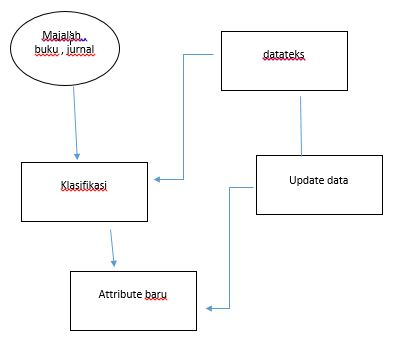
\includegraphics[width=4cm]{figures/1174003/4/klasifikasi.jpg}
            \centering
            \caption{Klasifikasi Text}
        \end{figure}

        \item Mengapa Klasifikasi Bunga tidak dapat menggunakan Machine Learning
        
        dikarenakan klasifikasi itu menggunakan tipe data yang dimana atributnya memiliki nilai data yang berupa vektor dengan perbandingan masing-masing data yang memiliki sedikit perbedaan. Dapat dilihat pada gambar berikut.
        \begin{figure}[H]
            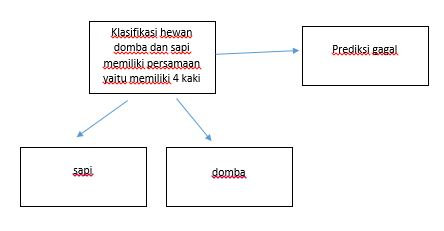
\includegraphics[width=4cm]{figures/1174003/4/hewan.jpg}
            \centering
            \caption{Klasifikasi Hewan}
        \end{figure}

        \item Teknik Pembelajaran maachine learning pada teks kata-kata di youtube
        
        Contohnya pada saat kita membuka sebuah video maka di sebelah kanan ada list "berikutnya", pada saat itu mesin melakukan ujicoba dan apabila anda menekan salah satu dari video tersebut maka hal tersebut akan direkam dan disimpan oleh mesin tersebut

        \begin{figure}[H]
            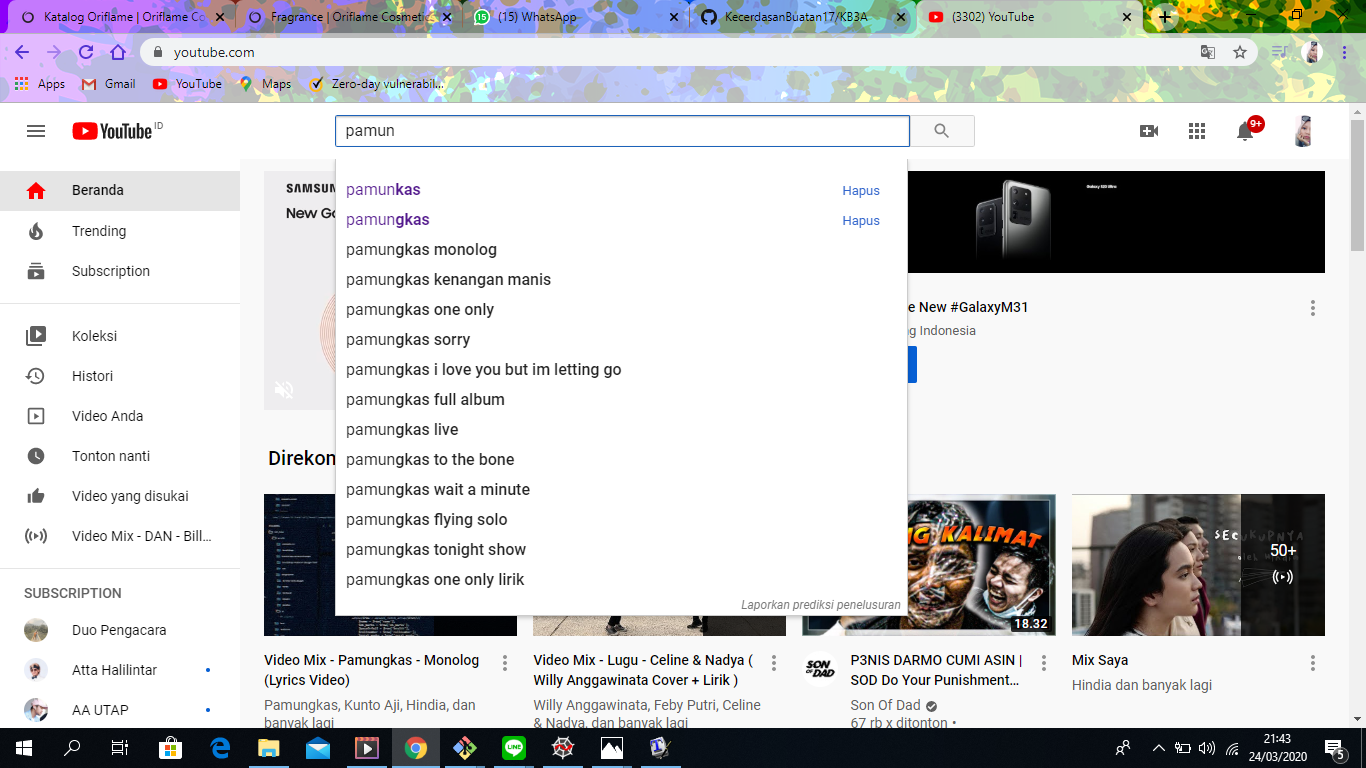
\includegraphics[width=4cm]{figures/1174003/4/youtube.jpg}
            \centering
            \caption{Machine Learning Youtube}
        \end{figure}

        \item Jelaskan apa yang dimaksud vektorisasi data.
        
        vektorisasi data merupakan pemechan data menjadi bagian bagian yang lebih sederhana contoh ada sebuah paragraf, dari paragraf tersebut akan dibagi bagi menjadi kalimat, yang nantinya akan dibagi bagi kembali menjadi perkata.

        \item Jelaskan apa itu bag of words dengan kata-kata yang sederhana dan ilustrasi sendiri
        
        Bag of words merupakan penyajian sederhana yang biasanya digunakan pada aplikasi text mining pada saat mengenalkan strukturke sebuah kumpulan dokumen yang berbasis teks untuk diklasifikasikan kembali menjadi dua atau lebih kelas yang telah di tentukan.

        \begin{figure}[H]
            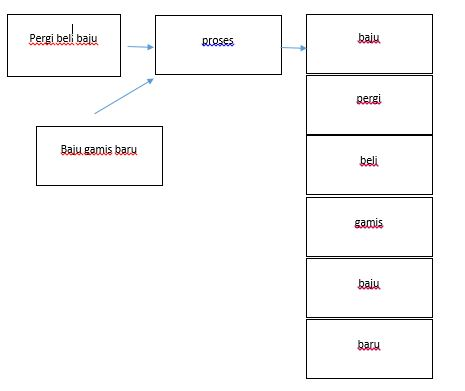
\includegraphics[width=4cm]{figures/1174003/4/baju.jpg}
            \centering
            \caption{Bag of Words}
        \end{figure}

        \item Jelaskan apa itu TF-IDF, ilustrasikan dengan gambar sendiri.
        
        TF-IDF merupakan metode untuk menghitung bobot dari kata yang sering muncul pada suatu kalimat. metode ini menghitung nilai Term Frequency dan IDF atau Inverse Document Frequency pada setiap kata pada kalimat yang dijadikan acuan kata pada metode ini sering di sebut token adapun rumus dari metode ini dapat dilihat pada gambar.
        \begin{figure}[H]
            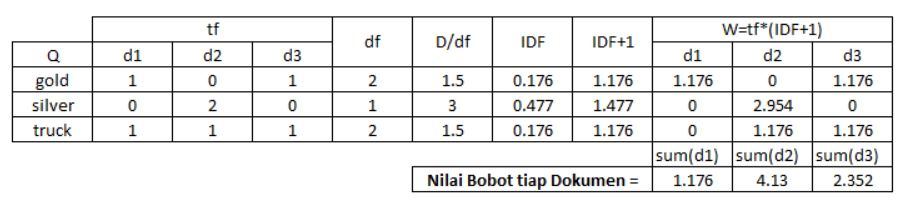
\includegraphics[width=4cm]{figures/1174003/4/tfidf.jpg}
            \centering
            \caption{TF-IDF}
        \end{figure}

    \end{enumerate}

    \subsection{Praktek}
    \begin{enumerate}
        \item import data pandas dan 500 baris data dumy kemudian di jelaskan tiap barisnya. 
\hfill \break \lstinputlisting[firstline=8, lastline=13]{src/1174003/4/praktek1.py}
        
        \begin{figure}[H]
            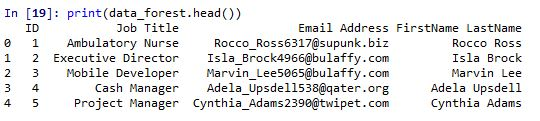
\includegraphics[width=4cm]{figures/1174003/4/1.jpg}
            \centering
            \caption{Data Dummy}
        \end{figure}

        \item memecah data prame menjadi dua yag pertama 450 dan kedua sisanya \hfill \break \lstinputlisting[firstline=14, lastline=16]{src/1174003/4/praktek2.py}
        
        \begin{figure}[H]
            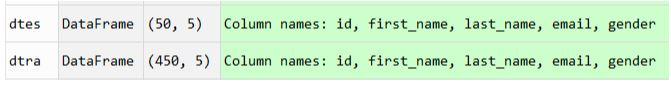
\includegraphics[width=4cm]{figures/1174003/4/2.jpg}
            \centering
            \caption{Pisah Data}
        \end{figure}

        \item praktek vektorisasi \hfill \break \lstinputlisting[firstline=17, lastline=47]{src/1174003/4/praktek2.py}
        
        lakukan import library pandas yang di inisialisasi menjasi pd setelah itu ada dibuat variable data dengan method read\_csv untuk membaca file berekstensikan csv yang di masukan alamatnya pada kurung, lakukan klasifikasi atau pemilihan komentar yang berisi spam atau bukan spam dengan parameter class samadengan 1 merupakan spam dan class samadengan 0 bukan spam setelah itu masukan librari CountVektorizer yang digunakan untuk vektorisasi data kemudian dilanjutkan pada bagian In[103] dibuat variabel yang berisi vektorisasi dari data pada data di field content setelah itu variabel tersebut di running hasilnya menunjukan 350 baris di kali 1738 kolom selanjutnya dicoba untuk memunculkan isi recod pada baris ke 345 maka akan muncul isian dari baris tersebut. selanjutnya dibuat variabel dk atau daftar yang berisi data hasil vektorisasi setelah yang terdiri dari variabel dshuf yang berisi data komen yang di dalamnya di buat random yang nantinya akan dibut data training dan data testing dengan ketentuan data training 300 dan data testing sebanyak 50 setelah itu data training di lakukan vektorisasi dan data testing juga dilakukan vektorisasi setelah itu kedua data training dan testing tersebut dibuat label dengan parameter field CLASS pada tabel.
        \begin{figure}[H]
            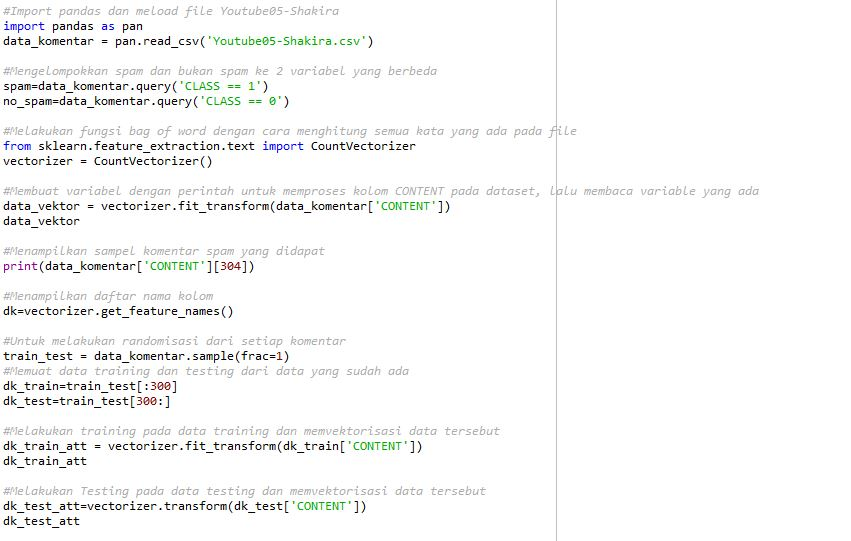
\includegraphics[width=4cm]{figures/1174003/4/3.jpg}
            \centering
            \caption{Vektorisasi}
        \end{figure}

        \item klasifikasi SVM \hfill \break \lstinputlisting[firstline=49, lastline=53]{src/1174003/4/praktek2.py}
        
        import librari svm dari sklearn kemudian membuat variabel clfsvm berisikan method svc setelah itu variabel tersebut di berikan method fit dengan isian data train vektorisasi dan data training label yang berguna untuk melatih data tersebut setelah itu di coba untuk memunculkan score atau akurasi dari data tersebut menggunakan data testing vektorisasi dan data testing label.
        \begin{figure}[H]
            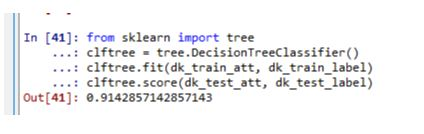
\includegraphics[width=4cm]{figures/1174003/4/4.jpg}
            \centering
            \caption{SVM}
        \end{figure}

        \item klasifikasi decision tree \hfill \break \lstinputlisting[firstline=55, lastline=58]{src/1174003/4/praktek2.py}
        
        import librari tree dari sklearn kemudian membuat variabel clftree berisikan method DecisionTreeClasifier setelah itu variabel tersebut di berikan method fit dengan isian data train vektorisasi dan data training label yang berguna untuk melatih data tersebut agar dapat digunakan pada codingan selanjutnya setelah itu di coba untuk memunculkan score atau akurasi dari data tersebut menggunakan data testing vektorisasi dan data testing label.
        \begin{figure}[H]
            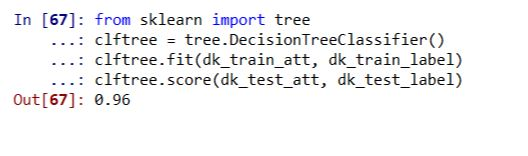
\includegraphics[width=4cm]{figures/1174003/4/5.jpg}
            \centering
            \caption{Desicion Tree}
        \end{figure}

        \item plot comfusion matrix \hfill \break \lstinputlisting[firstline=61, lastline=64]{src/1174003/4/praktek2.py}
        
        import library comfusion matrix selanjutnya dilakukan prediksi pada pada data tes nya kemudian data tersebut di masukan kedalam variabel cm dengan method confusion matrix yang di dalamnya terdapat data dari variabel perd label dan dk test label setelah itu variabel cm tersebut di running maka akan memunculkan nilai matrixnya. 
        \begin{figure}[H]
            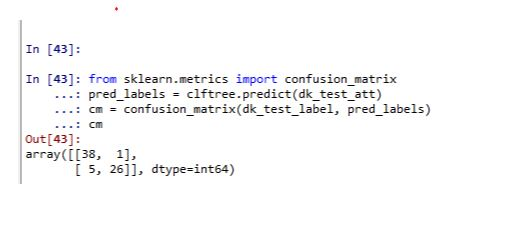
\includegraphics[width=4cm]{figures/1174003/4/6.jpg}
            \centering
            \caption{Confussion Matrix}
        \end{figure}

        \item cross valodation \hfill \break \lstinputlisting[firstline=66, lastline=85]{src/1174003/4/praktek2.py}
        
        memunculkan nilai akurasi dari tiga metode yaitu random forest, decision tree, dan klasifikasi svm (suport vector machine) diamana akan di bandingkan tingkat akurasi dari semua hasil akurasiya mana yang terbaik dan lebih akurat pada hasilnya data yang paling akurat yaitu random forest.
        \begin{figure}[H]
            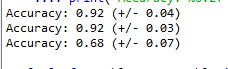
\includegraphics[width=4cm]{figures/1174003/4/7.jpg}
            \centering
            \caption{Cross Validation}
        \end{figure}

        \item Pengamatan program \hfill \break \lstinputlisting[firstline=88, lastline=104]{src/1174003/4/praktek2.py}
        
        terdapat grafik data yang terdapat dari grafik tersebut di dapat dari codingan dengan cara pengulangan data masing masing 10 kali setelah itu di eksekusi menjadi grafik berbentuk 3D pada gambar tersebut menunjukan rasio dari yang terrendah yaitu data SVM kemudian data decision tree dan hasil random forest.
        \begin{figure}[H]
            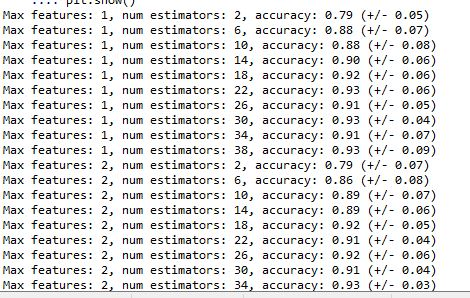
\includegraphics[width=4cm]{figures/1174003/4/8.jpg}
            \centering
            \caption{Pengamatan Program}
        \end{figure}

        Berikut adalah untuk grafik \hfill \break \lstinputlisting[firstline=108, lastline=122]{src/1174003/4/praktek2.py}
        \begin{figure}[H]
            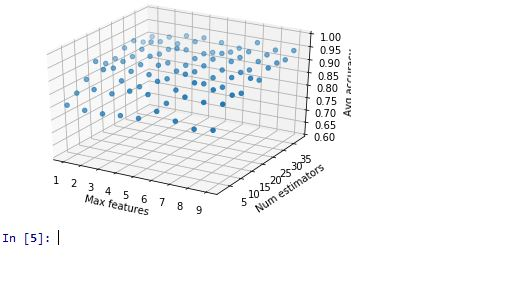
\includegraphics[width=4cm]{figures/1174003/4/9.jpg}
            \centering
            \caption{Grafik}
        \end{figure}
    \end{enumerate}
    \subsection{Penanganan Error}
        \subsubsection{Sreenshoot Error}
        \begin{enumerate}
            \item Error 1
            \begin{figure}[H]
                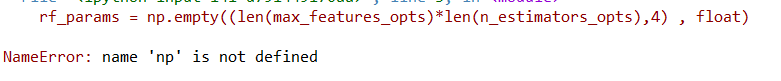
\includegraphics[width=4cm]{figures/1174003/4/errtype1.png}
                \centering
                \caption{Error1}
            \end{figure}
        \end{enumerate}
        \subsubsection{Kode Error dan Jenisnya}
        \begin{enumerate}
            \item Kode Error 1 jenis Name Error
            \begin{figure}[H]
                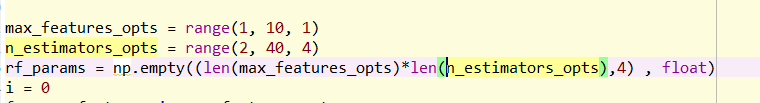
\includegraphics[width=4cm]{figures/1174003/4/err1.png}
                \centering
                \caption{Error1}
            \end{figure}
        \end{enumerate}
        \subsubsection{Solusi}
        \begin{enumerate}
            \item Mengimport liibrary numpy sebagai np
            \begin{figure}[H]
                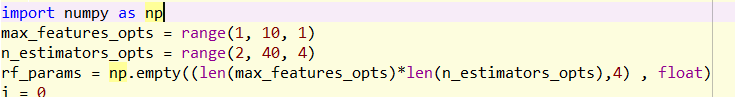
\includegraphics[width=4cm]{figures/1174003/4/solution1.png}
                \centering
                \caption{Solusi 1}
            \end{figure}
        \end{enumerate}